\documentclass[a4paper,12pt]{article}

%%% Работа с русским языком
\usepackage{cmap}					% поиск в PDF
\usepackage{mathtext} 				% русские буквы в формулах
\usepackage[T2A]{fontenc}			% кодировка
\usepackage[utf8]{inputenc}			% кодировка исходного текста
\usepackage[english,russian]{babel}	% локализация и переносы
\usepackage{xcolor}
\usepackage{hyperref}
 % Цвета для гиперссылок
\definecolor{linkcolor}{HTML}{799B03} % цвет ссылок
\definecolor{urlcolor}{HTML}{799B03} % цвет гиперссылок

\hypersetup{pdfstartview=FitH,  linkcolor=linkcolor,urlcolor=urlcolor, colorlinks=true}

%%% Дополнительная работа с математикой
\usepackage{amsfonts,amssymb,amsthm,mathtools} % AMS
\usepackage{amsmath}
\usepackage{icomma} % "Умная" запятая: $0,2$ --- число, $0, 2$ --- перечисление

%% Номера формул
%\mathtoolsset{showonlyrefs=true} % Показывать номера только у тех формул, на которые есть \eqref{} в тексте.

%% Шрифты
\usepackage{euscript}	 % Шрифт Евклид
\usepackage{mathrsfs} % Красивый матшрифт

%% Свои команды
\DeclareMathOperator{\sgn}{\mathop{sgn}}

%% Перенос знаков в формулах (по Львовскому)
\newcommand*{\hm}[1]{#1\nobreak\discretionary{}
{\hbox{$\mathsurround=0pt #1$}}{}}
% графика
\usepackage{graphicx}
\graphicspath{{pictures/}}
\DeclareGraphicsExtensions{.pdf,.png,.jpg}
\author{Бурмашев Григорий, БПМИ-208}
\title{Бурмашев, матан -- 8}
\date{\today}
\begin{document}
\maketitle
\section*{Номер 1}
\begin{center}
Имеем:
\end{center}
множество $D$ с разбиением $r = \{D_i\}$, причем $\Delta(r) < \delta$.
\begin{center}
Хотим:
\end{center}
каждое из $D_i \in r$ содержится внутри координатного куба с ребром $\delta$
\\\\
По определению:
\[
\Delta(r) = \underset{j}{\max} \; \underset{D_i}{\sup} |x - y| < \delta
\]
Отсюда:
\[
\underset{D_i}{\sup} |x - y| \leq \underset{j}{\max} \; \underset{D_i}{\sup} |x - y| < \delta \rightarrow D_i < \delta
\]
Предположим, что все таки не содержится в кубе с ребром $\delta$. Тогда сторона координатного куба будет $\geq \delta$. $|x - y|$ из формулы для $\Delta(r)$ будет диагональю куба, т.к это самое большое расстояние внутри куба (если сторона куба равна $a$, то диагональ $a \sqrt{3} > a$). Т.е если существует сторона с длиной $\geq \delta$, тогда диагональ тоже будет $\geq \delta$, тогда $\Delta(r) \geq \delta$, что есть \textbf{противоречие} изначальному условию про $\Delta(r) < \delta$ (т.е мы хотим, чтобы максимальное расстояние между двумя точками в нашей фигуре не превышало $\delta$, но при попытке рассмотреть случай с фигурой со стороной больше, чем $\delta$, все ломается, потому что $\Delta(r)$ будет $\geq$ $\delta$, т.к максимальное расстояние между двумя точками будет еще больше, чем сама сторона), а значит каждое из множеств $D_i$ содержится внутри координатного куба с ребром $\delta$
\begin{center}
\textbf{Ч.Т.Д} 
\end{center}
\clearpage
\section*{Номер 2}
\[
f(x) = \sin \left(\frac{1}{x}\right)
\]
Хотим отсутствие равномерной непрерывности на $(0, 1]$,  и при этом интегрируемость на этом же множестве.
\begin{itemize}
\item
Для интегрирумости нужно показать ограниченость и непрерывность на множестве:
\begin{enumerate}
\item
Сразу заметим, что наша функция ограничена, т.к  сам синус (очевидно) принимает значения от $-1$ до $1$.
\item
Функция также непрерывна, потому что наша функция является композицией функций $\sin x$ и $\frac{1}{x}$, а они, очевидно, непрерывны, отсюда получаем непрерывность $f(x) = \sin \left(\frac{1}{x}\right)$
\end{enumerate}
Отсюда получаем, что функция интегрируема по Риману
\item Разберемся с равномерной непрерывностью, по определению:
\begin{center}
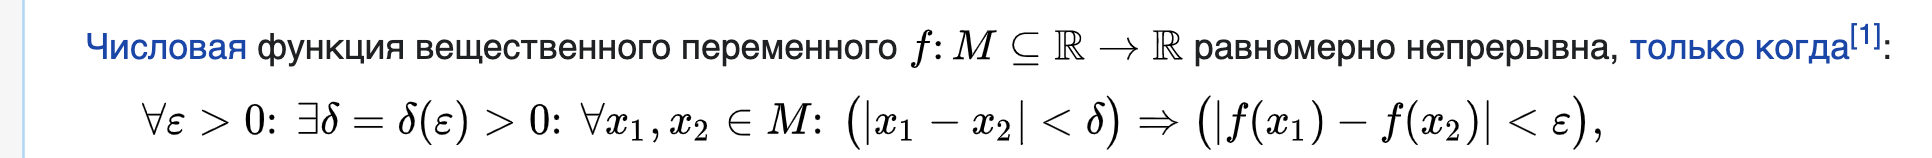
\includegraphics[scale=0.4]{1.png}
\end{center}
Покажем ее отсутствие, для этого посмотрим на отрицание для нашего случая ($M = (0, 1]$):
\[
\exists \varepsilon > 0 : \forall \delta > 0 : \exists \; x_1, x_2 \in M : |x_1 - x_2| < \delta   \rightarrow |f(x_1) - f(x_2)| \geq  \varepsilon
\]
\clearpage
Теперь посмотрим на график функции $\sin(\frac{1}{x})$:
\begin{center}
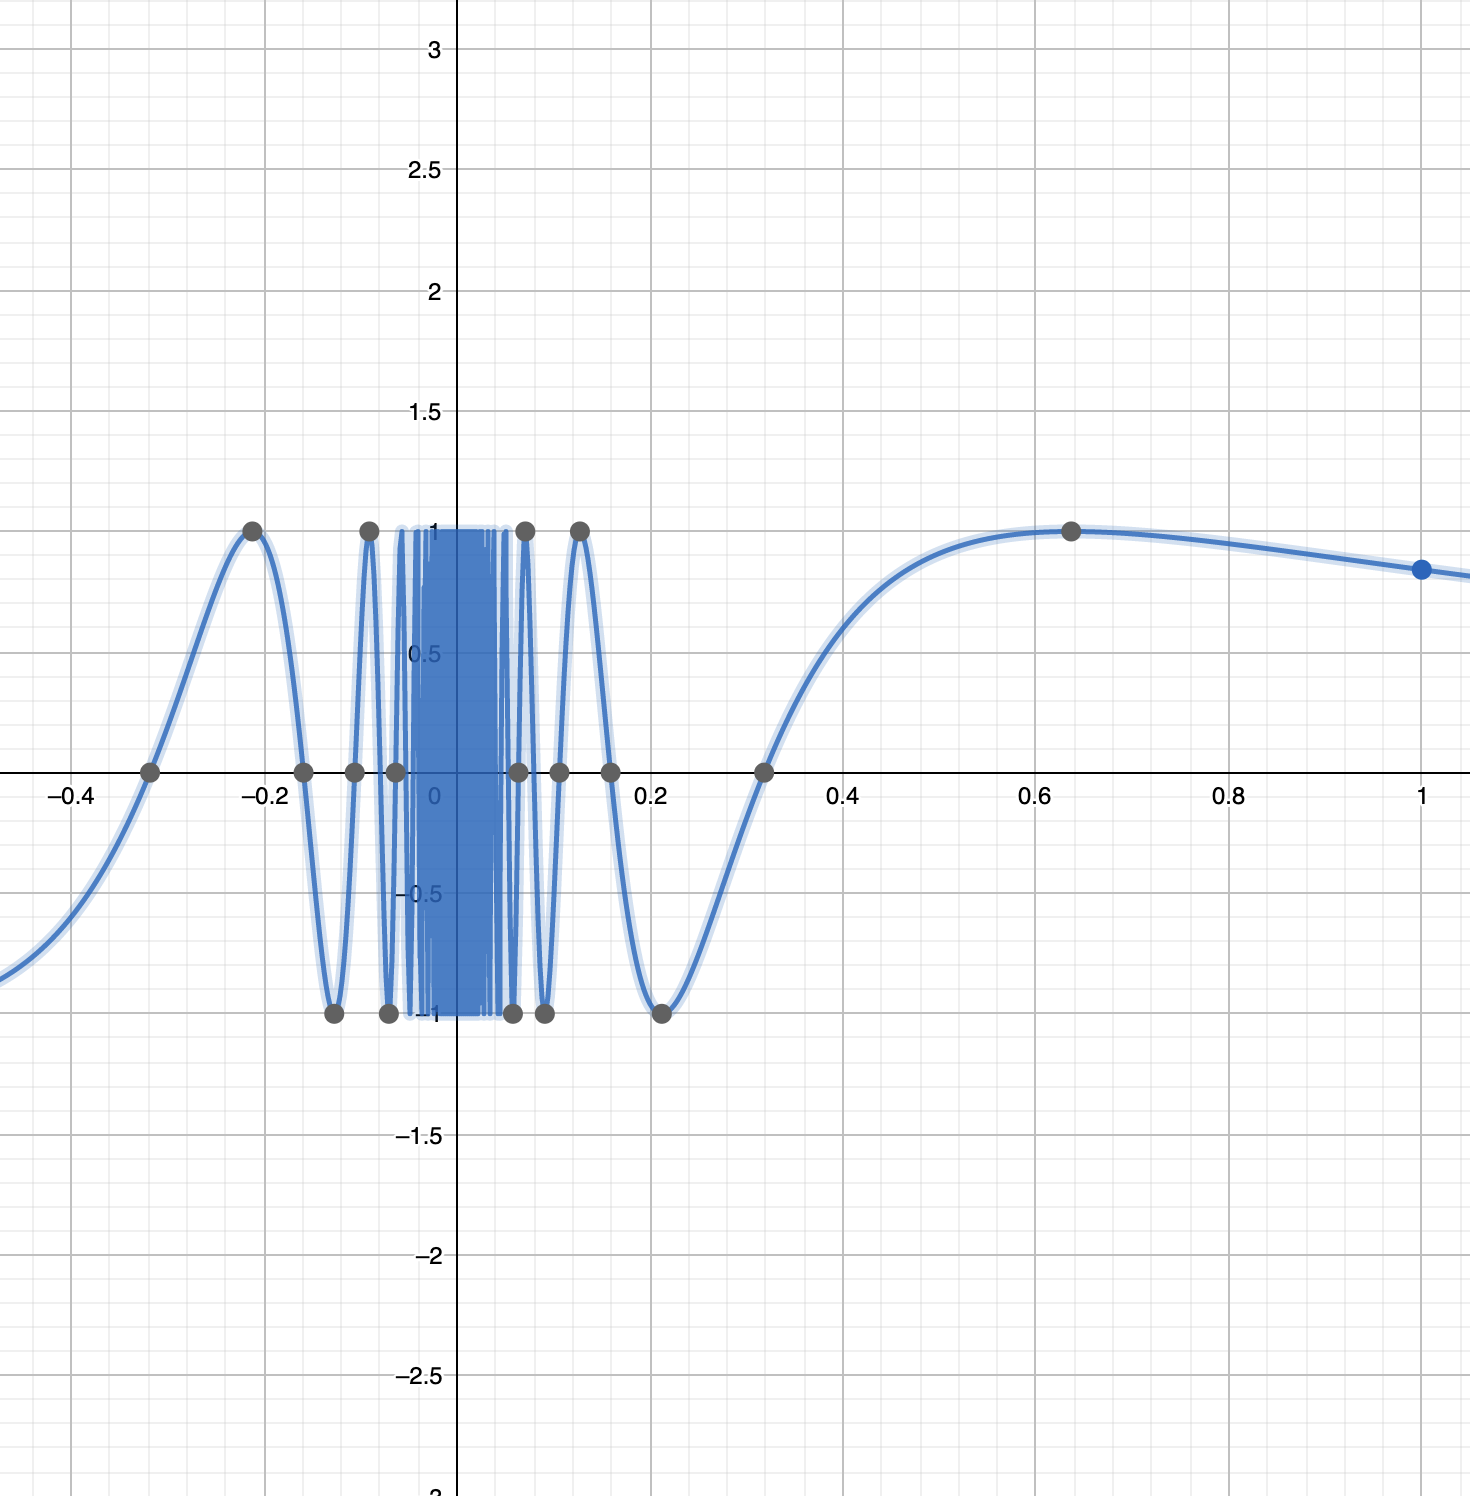
\includegraphics[scale=0.3]{2.png}
\end{center}
Не сложно заметить, что на $(0, 1]$ график функции достаточно сильно "мотает". Возьмем такие точки, в которых функция принимает значения $0$, $1$ и $-1$, мы можем это сделать удобно в рамках функции синуса (потому что знаем, что $\sin(\pi k) = 0, \sin(\frac{(2k+1)\pi}{2}) = \pm 1$)
\[
\frac{1}{x_1} = \pi k \rightarrow x_1 = \frac{1}{\pi k} \; \forall k \in \mathbb{N}
\]
\[
\frac{1}{x_2} = \frac{(2k + 1)\pi}{2} \rightarrow x_2 = \frac{2}{(2k+1)\pi} \forall k \in \mathbb{N}
\] 
Заметим, что $x_1, x_2 \in (0, 1]$

Теперь пытаемся выполнить условия для отрицания равномерной непрерывности:
\[
x_1 =  \frac{1}{\pi k} \underset{k \rightarrow \infty}{\longrightarrow} 0 
\]
\[
x_2 =  \frac{2}{(2k+1)\pi} \underset{k \rightarrow \infty}{\longrightarrow} 0 
\]
Отсюда получаем:
\[
|x_1 - x_2| \underset{k \rightarrow \infty}{\longrightarrow} 0 
\]
Т.е, взяв достаточно большой $k$, получаем, что:
\[
|x_1 - x_2| < \delta 
\]
Теперь посмотрим на значения функций:
\[
\sin(x_1) = 0 
\]
\[
\sin(x_2) = \pm 1
\]
Отсюда:
\[
|f(x_1) - f(x_2)| = |\sin(x_1)  - \sin(x_2)| = |\pm1| = 1 
\]
Теперь кладем $\varepsilon$ меньше единицы, и получаем выполнение отрицание равномерной непрерывности, другими словами, функция \textbf{не} является равномерно непрерывной
\end{itemize}
\begin{center}
\textbf{Ч.Т.Д} 
\end{center}
\end{document}
